\documentclass{article}
\usepackage[utf8]{inputenc}
\usepackage{graphicx}
\usepackage{hyperref}

\title{Installation Instruction for Vivado WebPack Edition}
\author{ECN-104 - Digital Logic Design }
\date{Spring 2018}

\begin{document}

\maketitle
\hypersetup{urlcolor=blue}
For this course we'll be using Xilinx's Vivado, Vivado is one of the most popular synthesis and HDL design tool. Xilinx provides Vivado WebPACK edition for free. Follow the instructions given below to create a new Xilinx account and install Vivado WebPACK edition on your computer. 

\section{Creating a new Xilinx account}
\begin{enumerate}
\item Go to \url{https://www.xilinx.com/registration/create-account.html} and create a new account.
\end{enumerate}

\section{Downloading the self-extracting installer}
\begin{enumerate}
\item Go to \url{https://www.xilinx.com/support/download.html}.
\item Under the section `\textit{Vivado Design Suite - HLx Editions - 2017.4  Full Product Installation}' choose the edition depending on your operating system.
\item If you are signed in, you will be forwarded to Xilinx's Name and Address verification page.
\item Enter your details here and click `\textit{Next}'.
\item If everything goes well Vivado installer would start getting downloaded.
\end{enumerate}

\section{Installing Vivado WebPACK Edition (on Windows)}
\begin{enumerate}
    \item Start the installer
    \item Enter your account details, select \textit{Download and Install Now} and press continue
    \item Agree to the terms and click next
    \item Choose `\textit{Vivado HL WebPACK}' and press continue
    \item Make the checklist on your screen matches Fig. \ref{Fig:install_options} and click next.
    \item Choose the installation location and press next
    \item Press install
\end{enumerate}

\begin{figure}[h] \centering 
  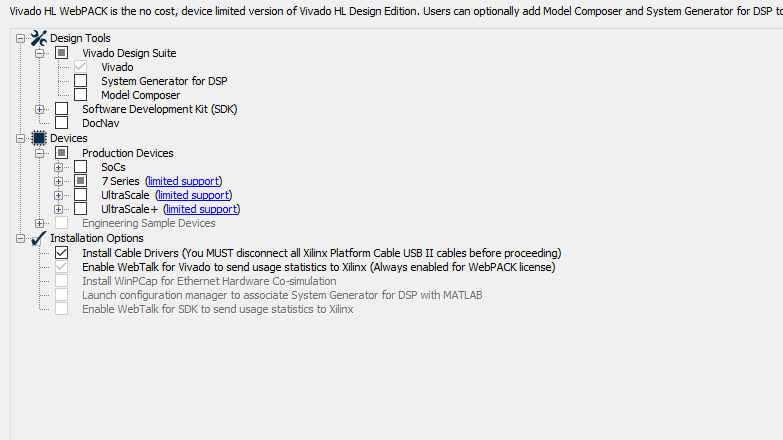
\includegraphics[width=\linewidth]{./images/install_options.png}
  \caption{Components to choose for installation of Vivado.}
  \label{Fig:install_options}
\end{figure}
The installer will now download and install all the required components.
\end{document}
